\section{Overhead}

One of our first concerns was to implement a framework that does not add an overhead to our simple application.
We have used the same setup than with our reference value and retrieve 1000 measurements to compute the overhead of our frameworks

\subsection{Extension framework overhead}

The extension framework have a large overhead of more than 2ms for with RE-Mote board and more than 3ms with the Z1 board.
On the figure \ref{fig:overhead-extension-contiki-z1}, we can see a side-by-side comparison of the two GPIO voltages without a framework on the left and with the extension framework on the right.
The comparison is shown with the Contiki on the Z1 board but the same overhead can be found with RIOT or with the RE-Mote board.
We explain later why our extension framework add such a latency.

% This latency is due to the way of how our framework output its measurements.
% Writting on the serial port is slow.
% Printing out at least 32 characters for every context switch on the serial port even at 250 kbit/s took 1.2ms.
% One optimization could be to reduce the number of bits send or use a cache.

\begin{figure}[!ht]
  \begin{minipage}{.45\textwidth}
      \centering
      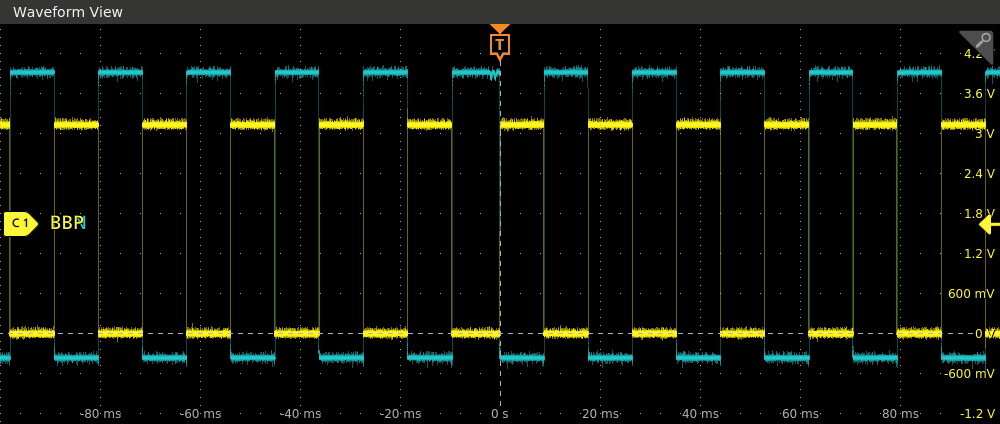
\includegraphics[scale=.25]{assets/reference-value-overhead-contiki-z1.png}
      \caption*{Voltage measurements with no framework}
  \end{minipage}\hfill
  \begin{minipage}{.45\textwidth}        
      \centering
      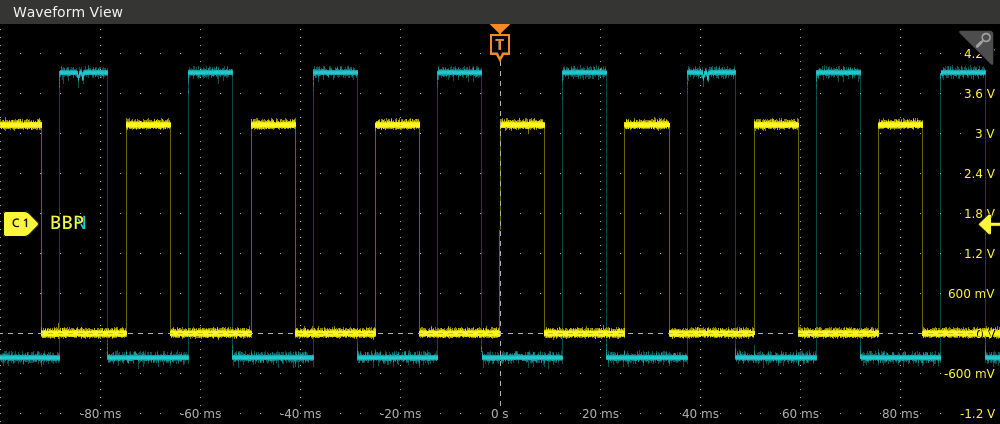
\includegraphics[scale=.25]{assets/extension-framework-overhead-contiki-z1.png}
      \caption*{Voltage measurements with the extension framework}
  \end{minipage}
  \caption{Overhead of the extension framework with Contiki on the Z1 \label{fig:overhead-extension-contiki-z1}}
\end{figure}

\subsection{Devices framework overhead}

The devices framework, in the other hand, have a small overhead of less than $3\mu s$ with either the RE-Mote or the Z1 boards.
The figure \ref{fig:overhead-devices-contiki-z1} shows the voltage measurements with Contiki on the Z1 board.
Both without the framework, on the left, and with the devices framework, on the right.
We compare later in this chapter why this devices framework have a small impact compared to our previous extension framework.

% As we do not use time-consumming methods, in contrary of the extension framework, the latency of the devices framework is much smaller than the latency of the extension framework.
% But even if the overhead is small, we must considerate it in our measurements.

\begin{figure}[!ht]
  \begin{minipage}{.45\textwidth}
      \centering
      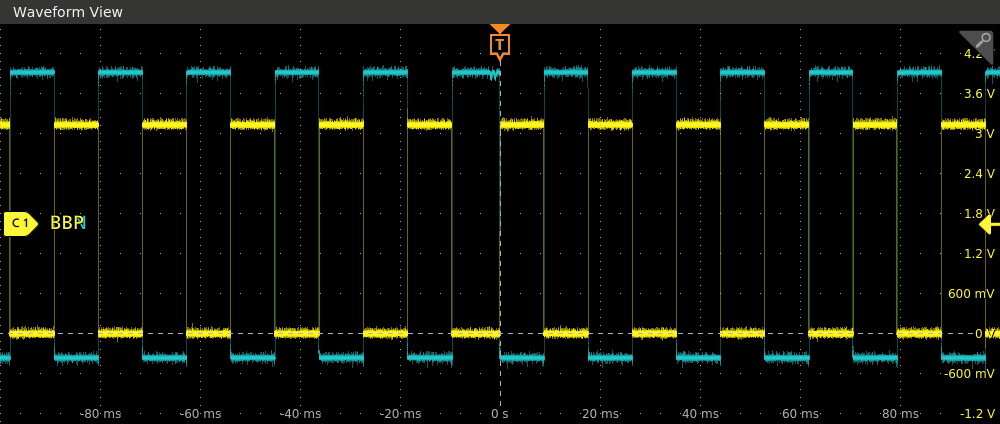
\includegraphics[scale=.25]{assets/reference-value-overhead-contiki-z1.png}
      \caption*{Voltage measurements with no framework}
  \end{minipage}\hfill
  \begin{minipage}{.45\textwidth}        
      \centering
      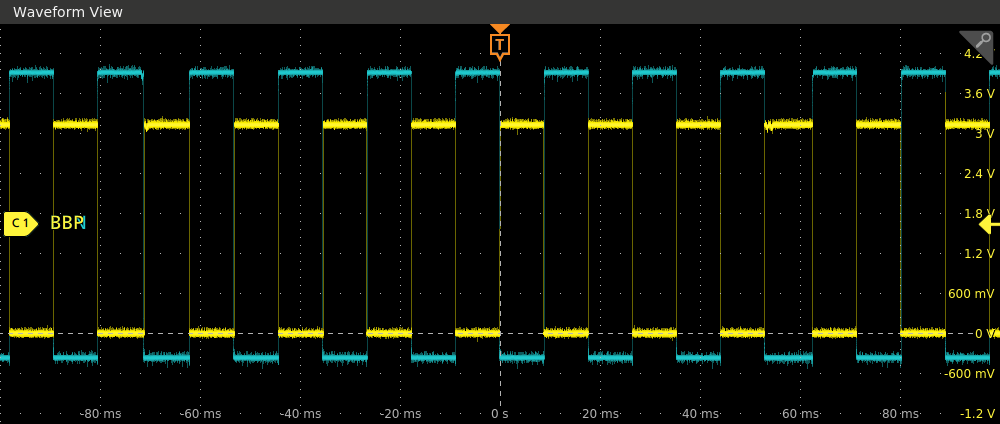
\includegraphics[scale=.25]{assets/devices-framework-overhead-contiki-z1.png}
      \caption*{Voltage measurements with the devices framework}
  \end{minipage}
  \caption{Overhead of the devices framework with Contiki on the Z1 \label{fig:overhead-devices-contiki-z1}}
\end{figure}